\documentclass{article}

\usepackage{arxiv}

\usepackage{hyperref}       % hyperlinks (but not footnotes: bug points links to titlepage)
\usepackage{url}            % simple URL typesetting
\usepackage{booktabs}       % professional-quality tables
\usepackage{amsfonts}       % blackboard math symbols
\usepackage[T1]{fontenc}	% font encoding
\usepackage{palatino}		% font typefaces
\usepackage{nicefrac}       % compact symbols for 1/2, etc.
\usepackage{microtype}      % microtypography
\usepackage{setspace}		% line spacing
\usepackage{etoolbox}		% for conditional statements
\AtBeginEnvironment{tabular}{\tiny}
\usepackage{lipsum}
\usepackage{graphicx}
\usepackage{tabularx}
\newcolumntype{s}{>{\hsize=.05\hsize}X}
\newcolumntype{m}{>{\hsize=.2\hsize}X}
\newcolumntype{l}{>{\hsize=.4\hsize}X}
\usepackage{pdflscape}
\usepackage{doi}
\renewcommand{\doitext}{}	% avoid "doi: doi:" in references lists

\usepackage{xcolor}

% References format
\usepackage[natbibapa]{apacite} % APA 6th ed. styling for citations and references list
\bibliographystyle{apacite}

%%
%% Circled numbers
%%
\usepackage{tikz}
\newcommand*\circled[1]{\tikz[baseline=(char.base)]{
	\scriptsize\node[shape=circle,draw,inner sep=1pt] (char) {#1};}}

%%
%% Line spacing
%%
\setstretch{1.32} 

\title{Discussion Scenarios}

\graphicspath{{./media/}}

\begin{document}
\maketitle

\section{Introduction}

We are focusing on the editorial process of an academic journal, which are typically published by large commercial publishing houses
(such as Elsevier, Springer Nature, Wiley, etc.). Such academic publishing houses typically publish several hundreds of journals.
They hire professional \textit{in-house} editorial staff to coordinate the editorial process for manuscripts, while external academic
editors (typically university professors) take the important editorial decisions on manuscripts based on peer-review comments. Peer-
review is the process of letting other experts in the field review and comment on a manuscript. Based on the results from peer-review,
the academic editor will make a decision on whether to accept for publication, reject, or request revisions to the manuscript. 
We are interested to explore and discuss why and how \textit{adaptive} and hybrid AI systems could help such a commercial publisher
\textit{to gain a competitive advantage} over other publishers. We focus on use cases that are \textit{hybrid and adaptive} and can
learn from the user, adapt to the user, or adapt to the environment (e.g., through continuous training / learning).

In the following you will find a short description of the editorial process of a journal, a simplified BPMN diagram of the same 
process, and a table that lists possible use cases for AI in each of the steps of the editorial process. The table also includes
a column that describes the adaptability aspect of the AI use cases. This should guide your discussion, but you are free to
come up with your own use cases and ideas how adaptive AI could be used in this process. Each of the 4 groups will work on a
different part of the process. Please only work on the part assigned to your group: the numbers refer to the number in BPMN diagram
in Figure ~\ref{fig:bpmnEditorialProcess} and in the Table ~\ref{tab:editorialProcess}. Please fill in the results from your
discussion in the PowerPoint template provided in the teams channel $>$ $Files$ $>$ $Workshop\_Didi$ $>$ $Group$\_$[1,2,3,4].pptx$

\subsection{Discussion Groups}

\begin{itemize}
    \item \textbf{Group 1} / author / step 1 -- writing the manuscript -- hint: how and why would a company offer an AI that adapts to the author to write a paper (think of writing your paper for Emerging Topics)?
    \item \textbf{Group 2} / author / steps 2-3 -- searching for journal, formatting -- hint: how and why would a company offer an AI to learn author's preferences (think of a recommender system like Netflix)?
    \item \textbf{Group 3} / editor / step 6 -- desk review of manuscript (ethical checks) -- hint, e.g., check the graphics on how ethical problems change over time \url{http://doi.org/10.1126/science.aav8384}
    \item \textbf{Group 4} / editor / step 7 -- searching for reviewers -- hint: focus e.g. on slides 11--12, 15--17, 20--21 \url{https://github.com/rordi/aaai-make-2023/blob/main/slides.pdf}
\end{itemize}


\section{Costs of the Editorial Process}

Figure ~\ref{fig:mdpiFinancials2021} shows that the editorial processing (incl. production such as typesetting and copy-editing) is the most
expensive aspect of publishing a journal. The processing of a manuscript costs ca. 800 CHF -- which includes the costs for processing manuscripts
that are finally rejected. A rejected manuscript does not generate any revenue for the publisher. In the case of open access publishers, the 
publisher cannot charge publication fees for a rejected article, while a subscription based publisher can not charge pay-per-view fees or 
create value for annual subscribers from rejected manuscripts. Figure ~\ref{fig:mdpiSubmissions2022} shows an example of data on manuscript
submissions and rejections.

\section{The Editorial Process}

A simplified, typical editorial process for a manuscript submitted to a journal -- from writing the manuscript to the final decision of
acceptance or rejection -- is shown in Figure ~\ref{fig:bpmnEditorialProcess}. The process includes at least three parties: the author who
writes the manuscript, the editor of the journal (or conference chair) that coordinates the peer-review process, and the peer-reviewers
that review and comment on a manuscript. For some journals the editor could be two persons: an academic editor, such as an \textit{Editor-in-Chief},
taking the decisions on manuscripts after peer-review, and an internal editorial staff coordinating the editorial process.

The typical editorial process involves several steps that must be completed in a particular order. First, the author writes the manuscript
with the research results. Once the manuscript is complete, the author searches for an appropriate journal to submit it to. Next, the author
formats the manuscript according to the specific instructions of the chosen journal, i.e., edit and format the Microsoft Word or \LaTeX~document
to fit the style of the journal and references style used. The author then submits the manuscript files to the journal for consideration and
peer-review. 

Once the journal receives the manuscript, the editor performs a desk review to assess whether the manuscript meets the journal's requirements
and stated scope. Desk review includes checking the manuscript for a number of ethical issues, including detecting plagiarism, checking for tortured
phrases (``paraphrased plagiarism''), generated / fake papers, biased or inappropriate language, off-topic references, fabricated or manipulated
images, potentially inappropriate authorship, controversial topics, etc. If the manuscript passes the desk review, the editor will search for potential
reviewers who have expertise in the manuscript's subject. Depending on the journal and publisher, this task could be performed by the editorial staff of
the journal or by an external academic editor. In cases where the editor is an academic editor, they will typically search for reviewers
themselves. In cases where the editor is an internal editorial staff, they will typically use a reviewer recommendation system to search
for potential reviewers. Reviewer candidates are typically selected based on their expertise, previous publications, and after checking 
their conflicts of interests (e.g., if they have co-authored a paper with the author in the past). The editor will then invite reviewers
that passed the screening to evaluate the manuscript, i.e., invite them to peer-review the manuscript. If the reviewers accept the invitation,
they will be granted access to the manuscript, read it and write a review report that details their feedback and recommendations (typically
split into a part addressed to authors, and another part addressed to the editors of the journal). 

After all review reports have been received, the editor will read and assess each one. Based on the reviews, the editor will make a first
decision on whether to accept, reject, or request revisions to the manuscript. If revisions are required, the author will revise the manuscript
according to the review reports and asked to resubmit the revised version to the journal. The editor will then check the revised manuscript
and make a final decision on whether to accept it for publication in the journal.



\begin{figure*}[htb]
    \centering
    \caption{Example of a cost breakdown in journal publishing (public data from: MDPI, Annual Report 2021).}
    \label{fig:mdpiFinancials2021}
    \includegraphics[width=0.75\linewidth]{figures/2021_mdpi_financials.pdf}
\end{figure*}

\begin{figure*}[htb]
    \centering
    \caption{Example of submission versus publication numbers in journal publishing (public data from: MDPI, Annual Report 2023).}
    \label{fig:mdpiSubmissions2022}
    \includegraphics[width=0.75\linewidth]{figures/2022_mdpi_submissions.pdf}
\end{figure*}


\begin{landscape}
    \begin{figure*}[htb]
        \centering
        \caption{
            A simplified, typical editorial process from writing the manuscript to the final decision of acceptance or
            rejection for publication (in BPMN 2.0). For better understanding, the process steps performed by outside parties 
            are also modelled and the process starts with the outside party (author) writing the manuscript. The numbers
            indicate the sequence flow of the process.
            \linebreak~
        }
        \label{fig:bpmnEditorialProcess}
        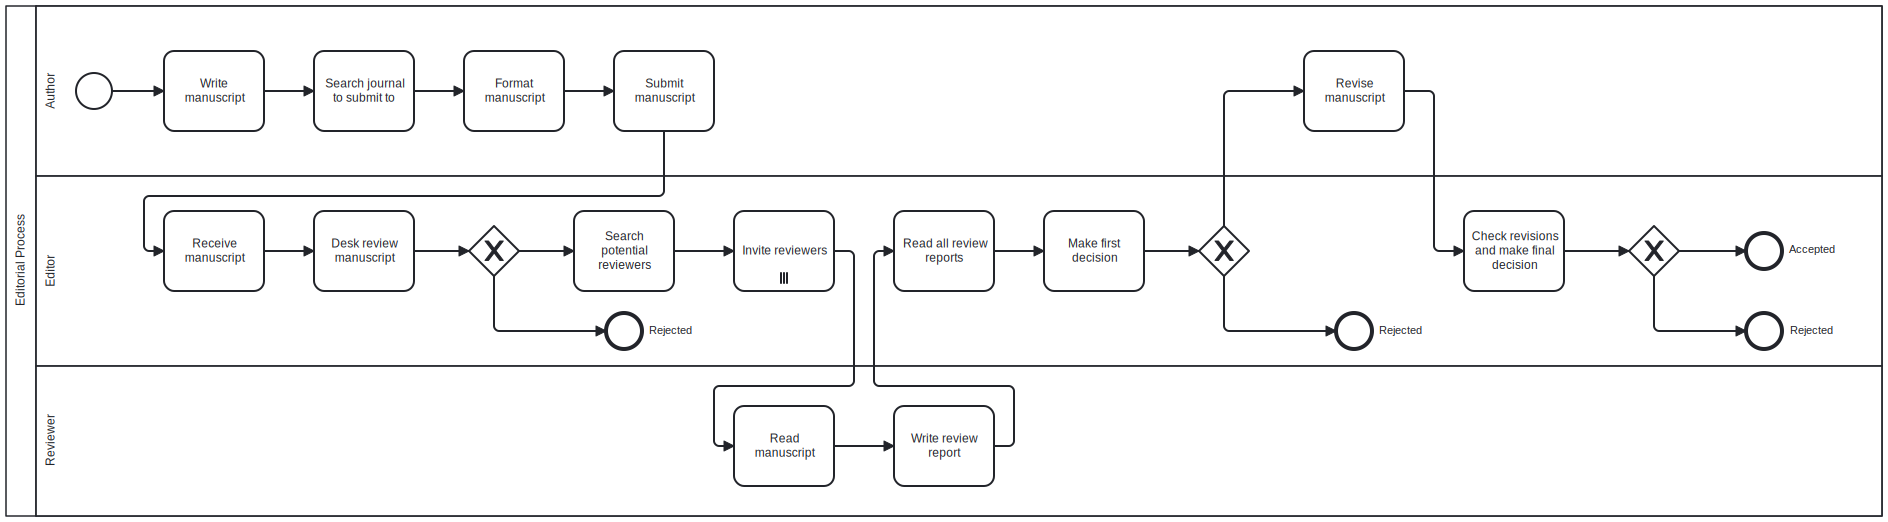
\includegraphics[width=\linewidth]{figures/editorial_process.pdf}
    \end{figure*}
\end{landscape}


\begin{landscape}
    \begin{table}[htb]
        \caption{
            Typical editorial processing steps and use cases for (hybrid) AI for a scholarly journal.
            \linebreak~
        }
        \label{tab:editorialProcess}

        \tiny
        \renewcommand{\arraystretch}{1.1}
        \small\centering
        \setlength\tabcolsep{8pt}
        \begin{tabularx}{\linewidth}{s m l X X}
            \toprule
            \textbf{Step} & \textbf{Role} & \textbf{Task} & \textbf{AI Use Cases} & \textbf{Adaptability Aspect} \\
            \midrule

            \circled{1} & Author & Writes manuscript & 
                Literature search, literature recommendation, summarization of key findings, writing (auto-completion), translating, grammar and spell-checking &
                AI adapts to user by learning what papers are relevant, recommends more similar papers, and expands to related concepts. \linebreak
                AI suggests auto-completions and corrections based on the \textit{user's writing style} and the context of the manuscript.
                \\ 

            \circled{2} & Author & Searches for journals to submit to & Journal recommendation &
                AI adapts to user by learning what journals are relevant to the user (journals read / cited, and journals previously published in)
                and recommends more similar journals.
                \\

            \circled{3} & Author & Formats paper to meet journal's requirements & Manuscript conversion and styling & 
                AI learns styles of journals and adapts its output to the journal selected by user \\

            \circled{4} & Author & Submits paper to a journal & Extraction of metadata & (Adaptability not required) \\

            \circled{5} & Editor & Receives manuscript submission & Summarization of key findings & (Adaptability not required) \\
            
            \circled{6} & Editor & Conducts desk review of the manuscript & Checks of the manuscript, including detecting plagiarism, tortured phrases
                ("paraphrased plagiarism"), generated papers, biased or inappropriate language, off-topic references, fabricated or manipulated images,
                potentially inappropriate authorship, controversial topics, etc. & AI needs to adapt to recent literature (e.g., plagiarism check needs
                to account for latest literature) and detecting new methods of generating papers.\\ 

            \circled{7} & Editor & Searches for potential reviewers & Semantic search (in vector space using word embeddings), graph embeddings,
                review assignment algorithms using e.g., knowledge graph to exclude potential reviewers with conflicts of interest & AI needs to
                adapt to recent literature and previous reviewer preferences of the editor \\ 

            \circled{8} & Editor & Invites potential reviewers to review & E-mail writing, generate summary of the manuscript &
                AI should learn the user's writing style and typical wording from previous examples. \\

            \circled{9} & Reviewer & Reads the manuscript & Summarization of key findings, checking of the content of cited references &
                AI needs to adapt to recent cited literature. \\ 

            \circled{10} & Reviewer & Writes review report & Writing (auto-completion) of qualitative review report: help reviewer to avoid biases,
                inappropriate feedback, lack of specificity & (Adaptability not required) \\ 

            \circled{11} & Editor & Reads all review reports & Checking of the quality of the peer-review report: detect biases, inappropriate 
                language, generic / non-specific feedback, ad hominem criticism, off-topic comments, etc.  & (Adaptability not required) \\ 

            \circled{12} & Editor & Makes decision on manuscript & Summarization of peer-review outcome for decision letter
                to author & AI should learn the user's writing style and typical wording from previous examples. \\ 

            \circled{13} & Author & Revises manuscript & Checking that reviewer concerns are being addressed, writing (auto-completion) of
                rebuttal letter to the reviewers \& editors & AI should learn the user's writing style and typical wording from previous examples. \\

            \bottomrule
        \end{tabularx}
    \end{table}
\end{landscape}

\end{document}